\documentclass[a4paper]{jsarticle}
\usepackage[dvipdfmx]{graphicx}
\usepackage{amsmath}
\usepackage{bm}
\renewcommand{\thesection}{第\arabic{section}問}
\renewcommand{\thesubsection}{(\arabic{subsection})}
\renewcommand{\thesubsubsection}{(\alph{subsubsection})}
\begin{document}

\title{2017分野3}
\author{nakao}
\maketitle

\section{}
\subsection{}
立方体1の鉛直方向の力のつり合いより、
\begin{equation}
  \rho_w r_1^2 h g = \rho_1 r_1^3 g
\end{equation}
が成り立ち、
\begin{equation}
  h = \frac{\rho_1}{\rho_w} r_1
\end{equation}
を得る。
また、左側の水槽の水面高さを$H_w + H_0$とする。
立方体1を入れる前後で左側の水槽の水の体積は変わらないから、
\begin{equation}
  A (H_w + H_0) - r_1^2 h = A H_w
\end{equation}
が成り立ち、
\begin{equation}
  H_0 = \frac{r_1^2 h}{A}
\end{equation}
を得る。
したがって、左側の水槽の水面高さは
$H_w + \frac{r_1^2 h}{A}$
である。
\subsection{}
X点とY点の圧力が等しくなる水位で静止するから、
\begin{equation}
  \rho_w g (H_w + H_0 - \eta_0)
  = \rho_w g (H_w + \eta_0)
\end{equation}
である。したがって、
\begin{equation}
  \eta_0 = \frac{H_0}{2} = \frac{r_1^2 h}{2 A}
\end{equation}
を得る。

\subsection{}
\subsubsection{}
静水圧分布として、
\begin{align}
  p_X &= \rho_w g (H_w + H_0 - \eta) \\
  p_Y &= \rho_g g (H_w + \eta)
\end{align}
である。

\subsubsection{}
\begin{equation}
  \frac{\partial u}{\partial t}
  = - \frac{1}{\rho} \frac{\partial p}{\partial x}
\end{equation}
が成り立つ。

\subsubsection{}
式(9)をXからYまで積分すると、
\begin{equation}
  \int_X^Y \frac{\partial u}{\partial t} \mathrm{d} x
  = \int_X^Y \left(-\frac{1}{\rho} \frac{\partial p}{\partial x}\right) \mathrm{d} x
\end{equation}
である。ここで、$u$は$x$依存しないから、
\begin{equation}
  \int_X^Y \frac{\partial u}{\partial t} \mathrm{d} x
  = \frac{\partial u}{\partial t} L
\end{equation}
であり、また、
\begin{equation}
  \int_X^Y \left(-\frac{1}{\rho} \frac{\partial p}{\partial x}\right) \mathrm{d} x
  = -\frac{1}{\rho} (p_Y - p_X)
  = (H_0 - 2 \eta) g
\end{equation}
である。したがって、
\begin{equation}
  \frac{\partial u}{\partial t} L
  = (H_0 - 2 \eta) g
\end{equation}
が成り立つ。

\subsubsection{}
管路への流入量と左側の水槽からの流出量が等しいから、
\begin{equation}
  u s = A \frac{\partial \eta}{\partial t}
\end{equation}
が成り立つ。

\subsubsection{}
式(14)より$u = \frac{A}{s} \frac{\partial \eta}{\partial t}$
であり、これと$\eta = \xi + \eta_0$を式(13)に代入すると、
\begin{equation}
  \frac{\partial^2 \xi}{\partial t^2}
  = -\frac{2 s g}{A L} \xi
\end{equation}
を得る。

\subsubsection{}
初期条件$\xi(0) = -\eta_0, \dot{\xi}(0) = 0$
のもとで式(15)を解くと、
\begin{equation}
  \xi = -\eta_0 \cos \sqrt{\frac{2 s g}{A L}} t
\end{equation}
を得る。これより、
\begin{equation}
  u = \frac{A}{s} \frac{\partial \eta}{\partial t}
  = \eta_0 \sqrt{\frac{2 A g}{s L}} \sin \sqrt{\frac{2 s g}{A L}} t
\end{equation}
となる。したがって、
\begin{align}
  U_0 &= \eta_0 \sqrt{\frac{2 A g}{s L}} \\
  \omega &= \sqrt{\frac{2 s g}{A L}}
\end{align}
である。

\subsubsection{}
$\eta_0, L$が$100$倍に、$A, s$が$100^2$倍になる。
このとき$U_0$は10倍になるから流速は10倍になる。
また、$\omega$が$1/10$倍になるから、周期は10倍になる。

\subsection{}
流速は$U_0 \sin \omega t$で表され、そのグラフは図1の通り。\par
抗力は、
\begin{equation}
  \begin{cases}
    \rho_w C_D r_2^2 U_0^2 \sin^2 \omega t & \left(0 \leq t \leq \frac{\pi}{\omega}\right) \\
    -\rho_w C_D r_2^2 U_0^2 \sin^2 \omega t & \left(\frac{\pi}{\omega} \leq t \leq \frac{2\pi}{\omega}\right) \\
  \end{cases}
\end{equation}
と表され、そのグラフは図2の通り。\par
慣性力は$\rho_w C_M r_2^3 U_0 \omega \cos \omega t$と表され、そのグラフは図3の通り。
\begin{figure}[htb]
  \begin{minipage}{0.3\hsize}
    \centering
    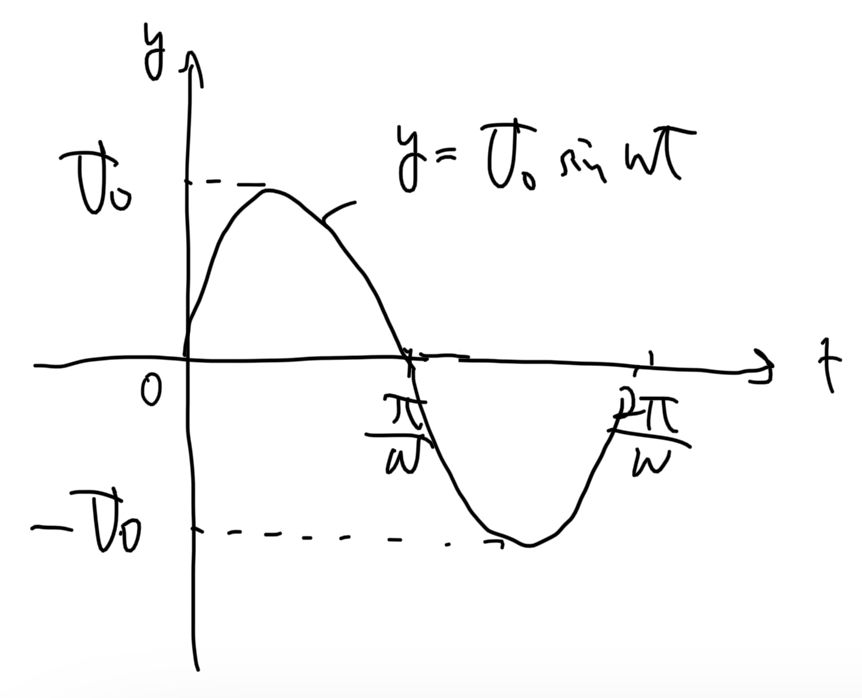
\includegraphics[width=\hsize]{fig1.png}
    \caption{流速の時系列}
  \end{minipage}
  \begin{minipage}{0.3\hsize}
    \centering
    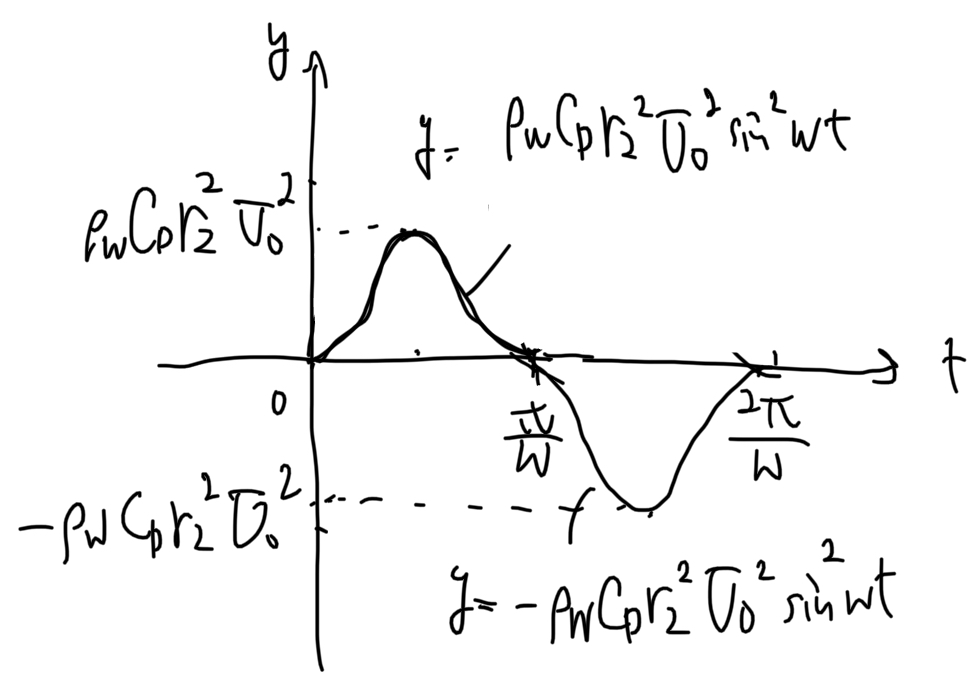
\includegraphics[width=\hsize]{fig2.png}
    \caption{抗力の時系列}
  \end{minipage}
  \begin{minipage}{0.3\hsize}
    \centering
    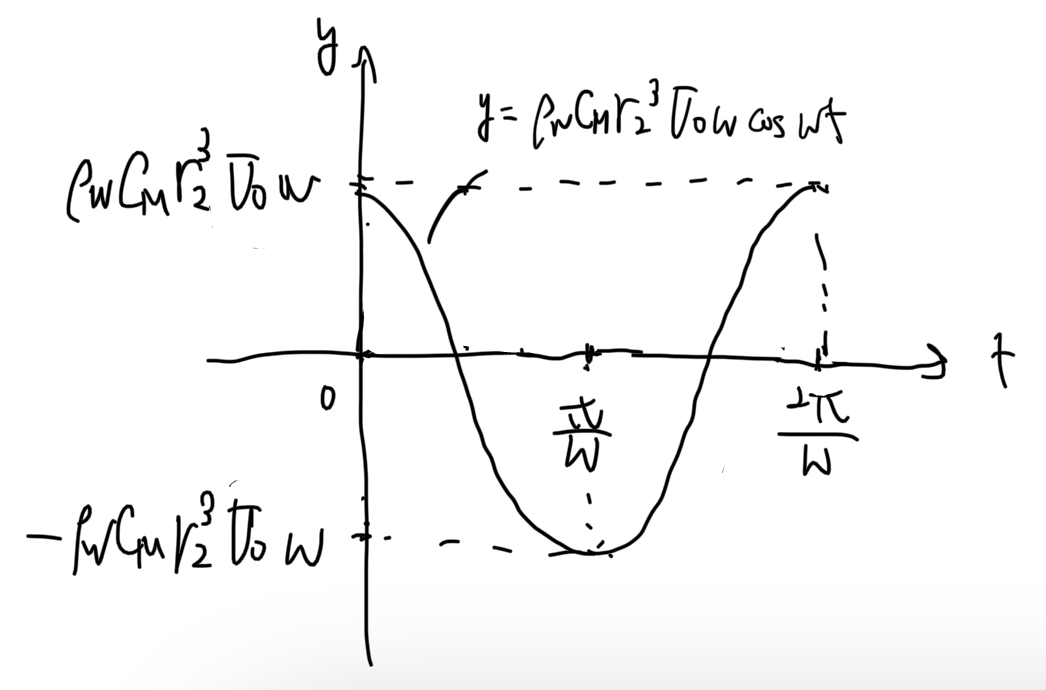
\includegraphics[width=\hsize]{fig3.png}
    \caption{慣性力の時系列}
  \end{minipage}
\end{figure}

\subsection{}
\subsubsection{}
式[2]より、$r_2$が2倍になったときに抗力は4倍、慣性力は8倍になる。
また、摩擦力は立方体2の質量に比例するため8倍になる。
したがって、立方体2は動かない。

\subsubsection{}
式(18)より、$L$を$1/2$倍にしたときに$U_0$は$\sqrt{2}$倍になる。
これを考慮すれば、$r_2$が2倍になったときに抗力は8倍、慣性力は$8\sqrt{2}$倍になる。
また、摩擦力は8倍になる。したがって、立方体2は動く。
\end{document}